% Created by tikzDevice version 0.6.2-92-0ad2792 on 2013-04-07 17:56:48
% !TEX encoding = UTF-8 Unicode
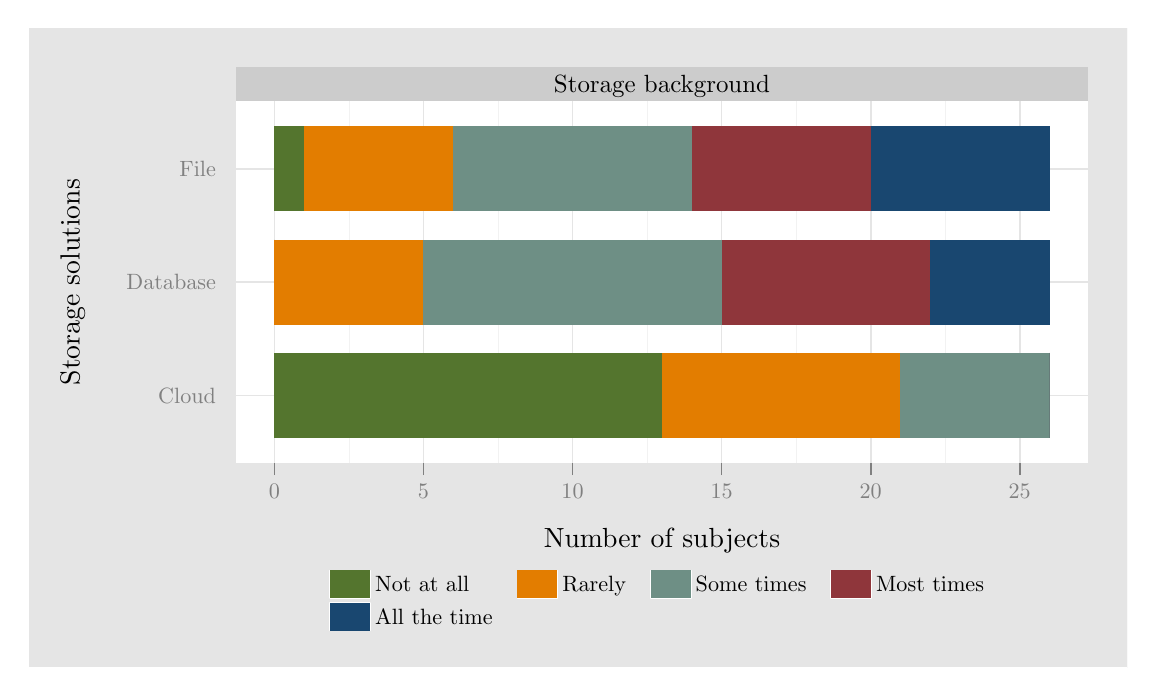
\begin{tikzpicture}[x=1pt,y=1pt]
\definecolor[named]{fillColor}{rgb}{1.00,1.00,1.00}
\path[use as bounding box,fill=fillColor,fill opacity=0.00] (0,0) rectangle (397.48,231.26);
\begin{scope}
\path[clip] (  0.00,  0.00) rectangle (397.48,231.26);
\definecolor[named]{drawColor}{rgb}{1.00,1.00,1.00}
\definecolor[named]{fillColor}{rgb}{0.90,0.90,0.90}

\path[draw=drawColor,line width= 0.6pt,line join=round,line cap=round,fill=fillColor] (  0.00,  0.00) rectangle (397.48,231.26);
\end{scope}
\begin{scope}
\path[clip] ( 75.16, 73.81) rectangle (383.26,204.82);
\definecolor[named]{fillColor}{rgb}{1.00,1.00,1.00}

\path[fill=fillColor] ( 75.16, 73.81) rectangle (383.26,204.82);
\definecolor[named]{drawColor}{rgb}{0.95,0.95,0.95}

\path[draw=drawColor,line width= 0.3pt,line join=round] (116.09, 73.81) --
	(116.09,204.82);

\path[draw=drawColor,line width= 0.3pt,line join=round] (169.96, 73.81) --
	(169.96,204.82);

\path[draw=drawColor,line width= 0.3pt,line join=round] (223.82, 73.81) --
	(223.82,204.82);

\path[draw=drawColor,line width= 0.3pt,line join=round] (277.68, 73.81) --
	(277.68,204.82);

\path[draw=drawColor,line width= 0.3pt,line join=round] (331.55, 73.81) --
	(331.55,204.82);
\definecolor[named]{drawColor}{rgb}{0.90,0.90,0.90}

\path[draw=drawColor,line width= 0.6pt,line join=round] ( 75.16, 98.38) --
	(383.26, 98.38);

\path[draw=drawColor,line width= 0.6pt,line join=round] ( 75.16,139.31) --
	(383.26,139.31);

\path[draw=drawColor,line width= 0.6pt,line join=round] ( 75.16,180.25) --
	(383.26,180.25);

\path[draw=drawColor,line width= 0.6pt,line join=round] ( 89.16, 73.81) --
	( 89.16,204.82);

\path[draw=drawColor,line width= 0.6pt,line join=round] (143.02, 73.81) --
	(143.02,204.82);

\path[draw=drawColor,line width= 0.6pt,line join=round] (196.89, 73.81) --
	(196.89,204.82);

\path[draw=drawColor,line width= 0.6pt,line join=round] (250.75, 73.81) --
	(250.75,204.82);

\path[draw=drawColor,line width= 0.6pt,line join=round] (304.62, 73.81) --
	(304.62,204.82);

\path[draw=drawColor,line width= 0.6pt,line join=round] (358.48, 73.81) --
	(358.48,204.82);
\definecolor[named]{fillColor}{rgb}{0.33,0.46,0.18}

\path[fill=fillColor] ( 89.16, 83.02) rectangle (229.21,113.73);
\definecolor[named]{fillColor}{rgb}{0.89,0.49,0.00}

\path[fill=fillColor] (229.21, 83.02) rectangle (315.39,113.73);
\definecolor[named]{fillColor}{rgb}{0.43,0.56,0.52}

\path[fill=fillColor] (315.39, 83.02) rectangle (369.25,113.73);
\definecolor[named]{fillColor}{rgb}{0.56,0.21,0.23}

\path[fill=fillColor] (369.25, 83.02) rectangle (369.25,113.73);
\definecolor[named]{fillColor}{rgb}{0.10,0.28,0.44}

\path[fill=fillColor] (369.25, 83.02) rectangle (369.25,113.73);
\definecolor[named]{fillColor}{rgb}{0.33,0.46,0.18}

\path[fill=fillColor] ( 89.16,123.96) rectangle ( 89.16,154.67);
\definecolor[named]{fillColor}{rgb}{0.89,0.49,0.00}

\path[fill=fillColor] ( 89.16,123.96) rectangle (143.02,154.67);
\definecolor[named]{fillColor}{rgb}{0.43,0.56,0.52}

\path[fill=fillColor] (143.02,123.96) rectangle (250.75,154.67);
\definecolor[named]{fillColor}{rgb}{0.56,0.21,0.23}

\path[fill=fillColor] (250.75,123.96) rectangle (326.16,154.67);
\definecolor[named]{fillColor}{rgb}{0.10,0.28,0.44}

\path[fill=fillColor] (326.16,123.96) rectangle (369.25,154.67);
\definecolor[named]{fillColor}{rgb}{0.33,0.46,0.18}

\path[fill=fillColor] ( 89.16,164.90) rectangle ( 99.93,195.61);
\definecolor[named]{fillColor}{rgb}{0.89,0.49,0.00}

\path[fill=fillColor] ( 99.93,164.90) rectangle (153.80,195.61);
\definecolor[named]{fillColor}{rgb}{0.43,0.56,0.52}

\path[fill=fillColor] (153.80,164.90) rectangle (239.98,195.61);
\definecolor[named]{fillColor}{rgb}{0.56,0.21,0.23}

\path[fill=fillColor] (239.98,164.90) rectangle (304.62,195.61);
\definecolor[named]{fillColor}{rgb}{0.10,0.28,0.44}

\path[fill=fillColor] (304.62,164.90) rectangle (369.25,195.61);
\end{scope}
\begin{scope}
\path[clip] (  0.00,  0.00) rectangle (397.48,231.26);
\definecolor[named]{fillColor}{rgb}{0.80,0.80,0.80}

\path[fill=fillColor] ( 75.16,204.82) rectangle (383.26,217.04);
\definecolor[named]{drawColor}{rgb}{0.00,0.00,0.00}

\node[text=drawColor,anchor=base,inner sep=0pt, outer sep=0pt, scale=  0.90] at (229.21,207.83) {Storage background};
\end{scope}
\begin{scope}
\path[clip] (  0.00,  0.00) rectangle (397.48,231.26);
\definecolor[named]{drawColor}{rgb}{0.50,0.50,0.50}

\node[text=drawColor,anchor=base east,inner sep=0pt, outer sep=0pt, scale=  0.80] at ( 68.04, 95.62) {Cloud};

\node[text=drawColor,anchor=base east,inner sep=0pt, outer sep=0pt, scale=  0.80] at ( 68.04,136.56) {Database};

\node[text=drawColor,anchor=base east,inner sep=0pt, outer sep=0pt, scale=  0.80] at ( 68.04,177.50) {File};
\end{scope}
\begin{scope}
\path[clip] (  0.00,  0.00) rectangle (397.48,231.26);
\definecolor[named]{drawColor}{rgb}{0.50,0.50,0.50}

\path[draw=drawColor,line width= 0.6pt,line join=round] ( 89.16, 69.54) --
	( 89.16, 73.81);

\path[draw=drawColor,line width= 0.6pt,line join=round] (143.02, 69.54) --
	(143.02, 73.81);

\path[draw=drawColor,line width= 0.6pt,line join=round] (196.89, 69.54) --
	(196.89, 73.81);

\path[draw=drawColor,line width= 0.6pt,line join=round] (250.75, 69.54) --
	(250.75, 73.81);

\path[draw=drawColor,line width= 0.6pt,line join=round] (304.62, 69.54) --
	(304.62, 73.81);

\path[draw=drawColor,line width= 0.6pt,line join=round] (358.48, 69.54) --
	(358.48, 73.81);
\end{scope}
\begin{scope}
\path[clip] (  0.00,  0.00) rectangle (397.48,231.26);
\definecolor[named]{drawColor}{rgb}{0.50,0.50,0.50}

\node[text=drawColor,anchor=base,inner sep=0pt, outer sep=0pt, scale=  0.80] at ( 89.16, 61.19) {0};

\node[text=drawColor,anchor=base,inner sep=0pt, outer sep=0pt, scale=  0.80] at (143.02, 61.19) {5};

\node[text=drawColor,anchor=base,inner sep=0pt, outer sep=0pt, scale=  0.80] at (196.89, 61.19) {10};

\node[text=drawColor,anchor=base,inner sep=0pt, outer sep=0pt, scale=  0.80] at (250.75, 61.19) {15};

\node[text=drawColor,anchor=base,inner sep=0pt, outer sep=0pt, scale=  0.80] at (304.62, 61.19) {20};

\node[text=drawColor,anchor=base,inner sep=0pt, outer sep=0pt, scale=  0.80] at (358.48, 61.19) {25};
\end{scope}
\begin{scope}
\path[clip] (  0.00,  0.00) rectangle (397.48,231.26);
\definecolor[named]{drawColor}{rgb}{0.00,0.00,0.00}

\node[text=drawColor,anchor=base,inner sep=0pt, outer sep=0pt, scale=  1.00] at (229.21, 43.46) {Number of subjects };
\end{scope}
\begin{scope}
\path[clip] (  0.00,  0.00) rectangle (397.48,231.26);
\definecolor[named]{drawColor}{rgb}{0.00,0.00,0.00}

\node[text=drawColor,rotate= 90.00,anchor=base,inner sep=0pt, outer sep=0pt, scale=  1.00] at ( 18.80,139.31) { Storage solutions};
\end{scope}
\begin{scope}
\path[clip] (  0.00,  0.00) rectangle (397.48,231.26);
\definecolor[named]{fillColor}{rgb}{0.90,0.90,0.90}

\path[fill=fillColor] (101.45,  9.15) rectangle (356.96, 39.41);
\end{scope}
\begin{scope}
\path[clip] (  0.00,  0.00) rectangle (397.48,231.26);
\definecolor[named]{drawColor}{rgb}{1.00,1.00,1.00}
\definecolor[named]{fillColor}{rgb}{1.00,1.00,1.00}

\path[draw=drawColor,line width= 0.6pt,line join=round,line cap=round,fill=fillColor] (109.33, 25.19) rectangle (123.79, 35.14);
\end{scope}
\begin{scope}
\path[clip] (  0.00,  0.00) rectangle (397.48,231.26);
\definecolor[named]{fillColor}{rgb}{0.33,0.46,0.18}

\path[fill=fillColor] (109.33, 25.19) rectangle (123.79, 35.14);

\path[] (109.33, 25.19) --
	(123.79, 35.14);
\end{scope}
\begin{scope}
\path[clip] (  0.00,  0.00) rectangle (397.48,231.26);
\definecolor[named]{drawColor}{rgb}{1.00,1.00,1.00}
\definecolor[named]{fillColor}{rgb}{1.00,1.00,1.00}

\path[draw=drawColor,line width= 0.6pt,line join=round,line cap=round,fill=fillColor] (176.95, 25.19) rectangle (191.40, 35.14);
\end{scope}
\begin{scope}
\path[clip] (  0.00,  0.00) rectangle (397.48,231.26);
\definecolor[named]{fillColor}{rgb}{0.89,0.49,0.00}

\path[fill=fillColor] (176.95, 25.19) rectangle (191.40, 35.14);

\path[] (176.95, 25.19) --
	(191.40, 35.14);
\end{scope}
\begin{scope}
\path[clip] (  0.00,  0.00) rectangle (397.48,231.26);
\definecolor[named]{drawColor}{rgb}{1.00,1.00,1.00}
\definecolor[named]{fillColor}{rgb}{1.00,1.00,1.00}

\path[draw=drawColor,line width= 0.6pt,line join=round,line cap=round,fill=fillColor] (225.14, 25.19) rectangle (239.59, 35.14);
\end{scope}
\begin{scope}
\path[clip] (  0.00,  0.00) rectangle (397.48,231.26);
\definecolor[named]{fillColor}{rgb}{0.43,0.56,0.52}

\path[fill=fillColor] (225.14, 25.19) rectangle (239.59, 35.14);

\path[] (225.14, 25.19) --
	(239.59, 35.14);
\end{scope}
\begin{scope}
\path[clip] (  0.00,  0.00) rectangle (397.48,231.26);
\definecolor[named]{drawColor}{rgb}{1.00,1.00,1.00}
\definecolor[named]{fillColor}{rgb}{1.00,1.00,1.00}

\path[draw=drawColor,line width= 0.6pt,line join=round,line cap=round,fill=fillColor] (290.35, 25.19) rectangle (304.81, 35.14);
\end{scope}
\begin{scope}
\path[clip] (  0.00,  0.00) rectangle (397.48,231.26);
\definecolor[named]{fillColor}{rgb}{0.56,0.21,0.23}

\path[fill=fillColor] (290.35, 25.19) rectangle (304.81, 35.14);

\path[] (290.35, 25.19) --
	(304.81, 35.14);
\end{scope}
\begin{scope}
\path[clip] (  0.00,  0.00) rectangle (397.48,231.26);
\definecolor[named]{drawColor}{rgb}{1.00,1.00,1.00}
\definecolor[named]{fillColor}{rgb}{1.00,1.00,1.00}

\path[draw=drawColor,line width= 0.6pt,line join=round,line cap=round,fill=fillColor] (109.33, 13.42) rectangle (123.79, 23.38);
\end{scope}
\begin{scope}
\path[clip] (  0.00,  0.00) rectangle (397.48,231.26);
\definecolor[named]{fillColor}{rgb}{0.10,0.28,0.44}

\path[fill=fillColor] (109.33, 13.42) rectangle (123.79, 23.38);

\path[] (109.33, 13.42) --
	(123.79, 23.38);
\end{scope}
\begin{scope}
\path[clip] (  0.00,  0.00) rectangle (397.48,231.26);
\definecolor[named]{drawColor}{rgb}{0.00,0.00,0.00}

\node[text=drawColor,anchor=base west,inner sep=0pt, outer sep=0pt, scale=  0.80] at (125.59, 27.41) {Not at all $\;\;$};
\end{scope}
\begin{scope}
\path[clip] (  0.00,  0.00) rectangle (397.48,231.26);
\definecolor[named]{drawColor}{rgb}{0.00,0.00,0.00}

\node[text=drawColor,anchor=base west,inner sep=0pt, outer sep=0pt, scale=  0.80] at (193.21, 27.41) {Rarely $\;\;$};
\end{scope}
\begin{scope}
\path[clip] (  0.00,  0.00) rectangle (397.48,231.26);
\definecolor[named]{drawColor}{rgb}{0.00,0.00,0.00}

\node[text=drawColor,anchor=base west,inner sep=0pt, outer sep=0pt, scale=  0.80] at (241.40, 27.41) {Some times $\;\;$};
\end{scope}
\begin{scope}
\path[clip] (  0.00,  0.00) rectangle (397.48,231.26);
\definecolor[named]{drawColor}{rgb}{0.00,0.00,0.00}

\node[text=drawColor,anchor=base west,inner sep=0pt, outer sep=0pt, scale=  0.80] at (306.61, 27.41) {Most times $\;\;$};
\end{scope}
\begin{scope}
\path[clip] (  0.00,  0.00) rectangle (397.48,231.26);
\definecolor[named]{drawColor}{rgb}{0.00,0.00,0.00}

\node[text=drawColor,anchor=base west,inner sep=0pt, outer sep=0pt, scale=  0.80] at (125.59, 15.64) {All the time $\;\;$};
\end{scope}
\end{tikzpicture}
